\chapter{Wing Box model} \label{chap:Model}

\section{Introduction} \label{sec:intro_Model}

% Introduction to the chapter

\section{Concept} \label{sec:concept_Model}

% Explanation of the concept
% -> Bending-twist coupling
% -> Shiftable shear centre location
% -> A web with variable-stiffness capability

% Figure: Fig. 1 Raither ?, Geometry and system of coordinates.
% Figure: Fig. 2 Raither ?, Schematic of the working principle.

% -> Buckling phenomena
% Figure: Schematic representation buckling phenomena

\section{Analytical model} \label{sec::analytical_Model}

%% Analytical apprach description
% An analytical model of the Wing Box will be build.
% Shear centre calculation
% The twist of the beam will be calculated
%
%Figure of analytical model
\begin{figure}[!htpb]
  \centering
  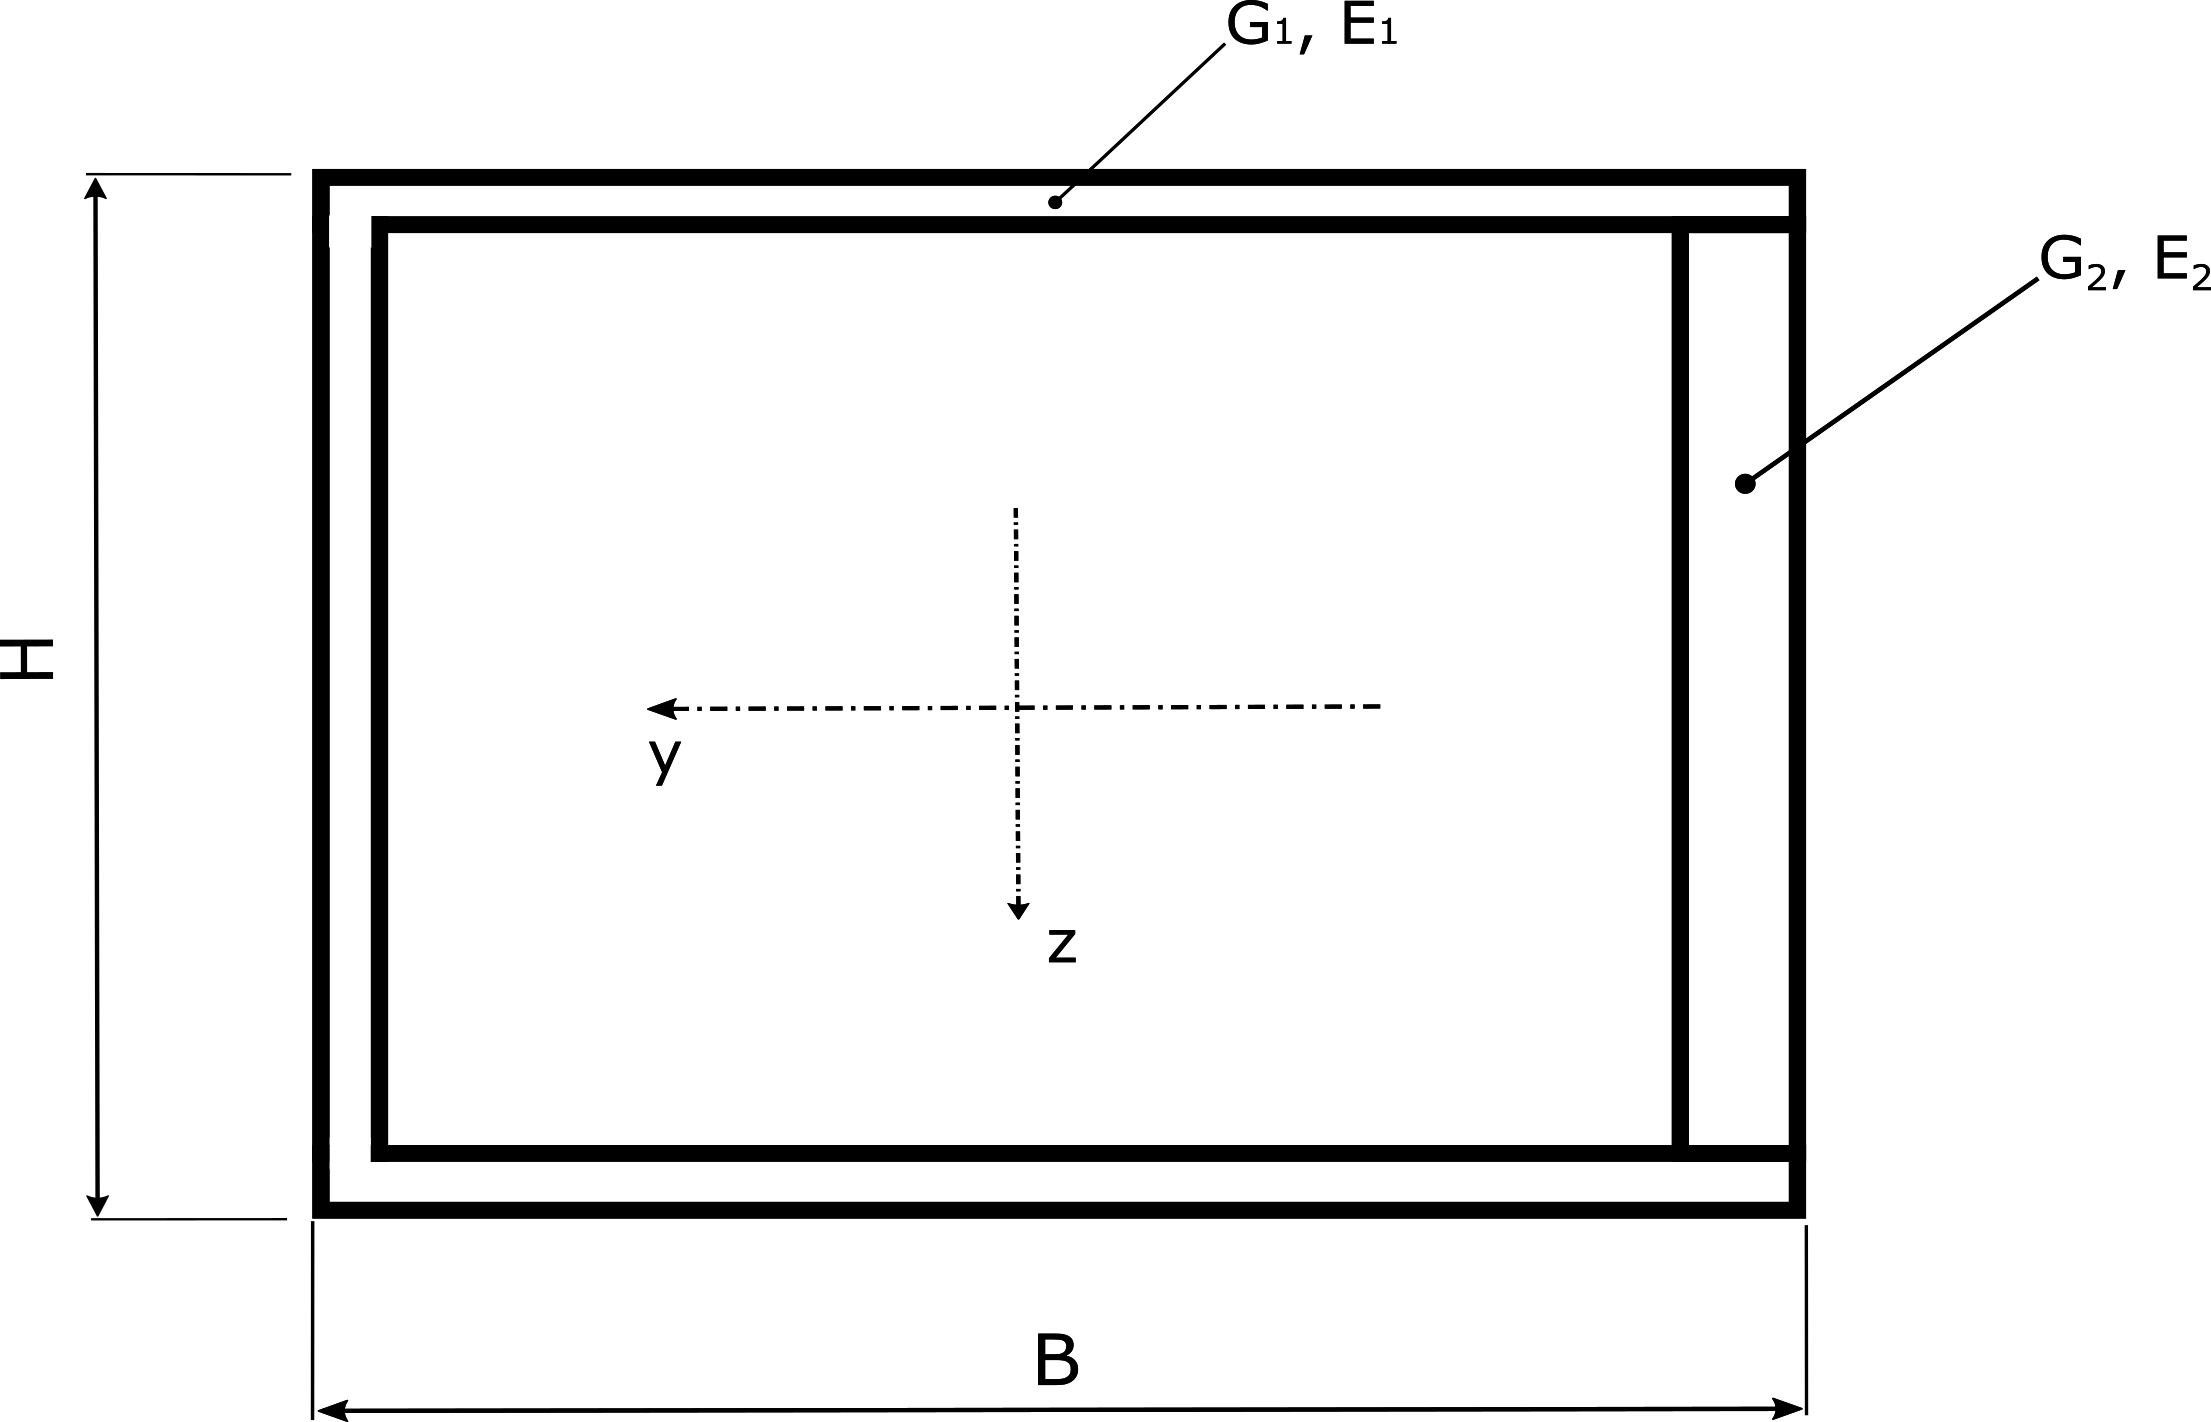
\includegraphics[width=0.8 \textwidth]{model/analyticalBox}
  \caption[Schematic view of the beam closed section]{Schematic view of the beam closed section. The dimensions are given by the width $B$ and the height $H$. For the upper, lower and left elements, the shear modulus and the elastic modulus are given by $G_1$ and $E_1$, respectively. For the right element, the same mechanical properties are given by $G_2$ and $E_2$.}\label{fig:analyticalBox}
\end{figure}

%Torsional stiffness

\begin{equation}\label{eq:torStiff}
  G I_t = \frac{4 A_0^2}{\oint \frac{\mathrm{d} s}{G(s) t(s)}}
\end{equation}

%Equations for the static moment and the flexural stiffness along the $y$ axis $\Phi_y$ (3.17, 3.18, 3.19)
Furthermore, the shear flow distribution in the beam will be calculated. In other to consider this distribution, the profile can be considered to be cut at one point, resulting on a opened section. The shear flow $q_{\parallel}(s)$ for this case can be calculated using Equation \ref{eq:shearFlowEquation}. The corresponding shear flow for a closed section can be obtained using the Equation \ref{eq:shearFlowDescomposition}.
%
\begin{equation}\label{eq:shearFlowEquation}
  q_{\parallel}(s) = - \frac{Q_z}{\Phi_y} S_{E_y}(s)
\end{equation}
%
\begin{equation}\label{eq:shearFlowDescomposition}
  q_\mathrm{C}(s) = q_\parallel(s) + q_0 
\end{equation}
%
where $Q_z$ is the force applied in the z direction and $\Phi_y$ is the flexural stiffness given by Equation \ref{eq:flexuralStiffness}. Additionally, $S_{E_y}$ is the so called static moment or first moment of area, which is calculated through the integral shown in Equation \ref{eq:staticMoment}. Also, the variable $q_0$ represents the shear flow at the boundary that results from the torsion of the beam and can be calculated using the Equation \ref{eq:constantShearFlow}.
%
\begin{equation}\label{eq:flexuralStiffness}
  \Phi_y = \int \int E(y,z) z^2 \mathrm{d}y \mathrm{d}z
\end{equation}
%
\begin{equation}\label{eq:staticMoment}
  S_{E_y}(s) = \int_0^s E(s) t(s) z(s) \mathrm{d}s
\end{equation}
%
\begin{equation}\label{eq:constantShearFlow}
  q_0 = \frac{Q_z}{\Phi_y} \frac{ \oint_s \frac{S_{E_y}(s)}{G(s) t(s)} \mathrm{d}s }{ \oint_s \frac{1}{G(s) t(s)} \mathrm{d}s }
\end{equation}

Now, the shear centre position in the beam transversal section will be calculated for the case of open section. Given that beam mechanical properties and geometrical dimensions are symmetric around y axis, the shear centre position in the z axis will be $z_{\mathrm{SC}} = 0$. On the other hand, the shear centre position in the y axis will be given by the Equation \ref{eq:shearCentrePosition}.
%
\begin{equation}\label{eq:shearCentrePosition}
  y_{\mathrm{SC,open}} = \frac{1}{Q_z} \oint_s q_\mathrm{C}(s) r(s) \mathrm{d}s
\end{equation}
%
where $r$ represents the perpendicular distance to the coordinate origin.

Now, it is necessary that equilibrium exists between the torsional moment due to the shift of the shear centre (caused during the opening of the profile) and the moment due to the torsional shear flow of the closed profile. This condition can be mathematically expressed through Equation \ref{eq:shearCentrePositionMoment}.
%
\begin{eqnarray}\label{eq:shearCentrePositionMoment}
% \nonumber % Remove numbering (before each equation)
  M_\mathrm{t} &=& Q_\mathrm{z} (y_{\mathrm{SC,open}} - y_{\mathrm{SC,closed}}) \nonumber \\
  &=& 2 A_0 q_0
\end{eqnarray}
%
%where it has been considered that a positive moment $M_\mathrm{t}$ along the x direction produces a constant shear flow distribution which has negative sign given the shear flow distribution definition in the present text.

Finally, the total shear flow $q(s)$ results from the superposition of the shear flow of the open profile $q_\mathrm{C}$ and the constant shear flow due to torsion $q_0$, as shown in the Equation \ref{eq:totalShearFlow}.
%
\begin{equation}\label{eq:totalShearFlow}
  q(s) = q_\mathrm{C}(s) - q_0 %before it was: q_\mathrm{C}(s) - q_\mathrm{M}
\end{equation}

\section{Computational model} \label{sec:computationalModel}

% Description of the model
%   Include all the parts of the model: C-box shape, inner box, chiral lattice
%   Figure of the model
% Parameters included
%
The computational model of the wing box was build using Abaqus CAE commercial software. It consisted on three main elements: the wing-box with C-profile, the lattice constituted of the chiral elements, a closed rib at the tip of the box and a closed rib at the root of the box. A general overview of the assembly of the different parts can be seen in Figure \ref{fig:all-assembly}.

\begin{figure}[!htpb]
  \centering
  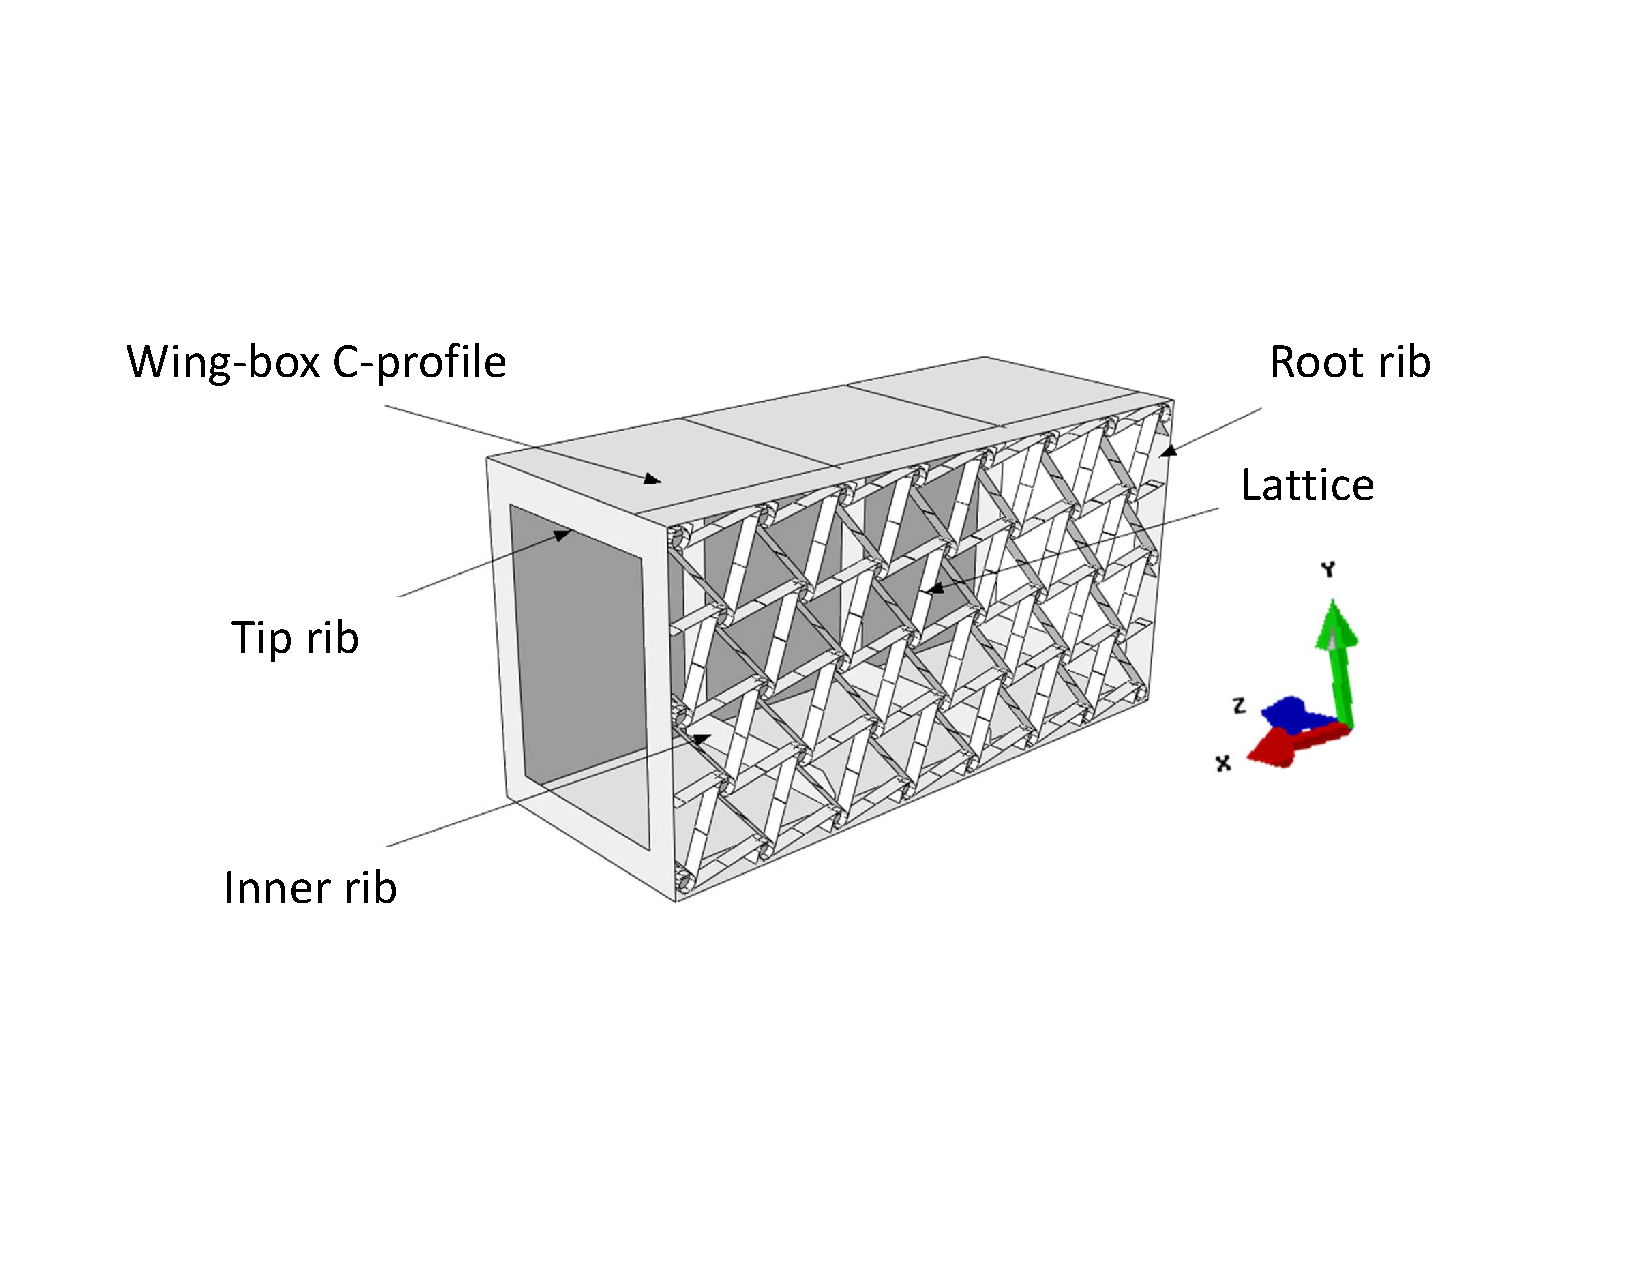
\includegraphics[width=0.8 \textwidth]{model/all-assembly}
  \caption[General assembly configuration for the computational model]{General assembly configuration for the computational model. The different parts for the general configuration include the wing-box profile, the lattice and the pair of ribs located at the tip and the root of the wing-box.}\label{fig:all-assembly}
\end{figure}

\subsection{Sub-parts and parametrization of the model} \label{subsec:parametrization_Model}

\subsubsection{Lattice of chiral elements} \label{subsubsec:lattice_Parametrization}

The model of the lattice structure is constituted of a series of interconnected lattices and nodes. An overview of the corresponding part can be seen in Figure \ref{fig:lattice}. The parameters used to characterize the element are shown in Table \ref{tab:parameters_lattice}. 

\begin{figure}[!htpb]
  \centering
  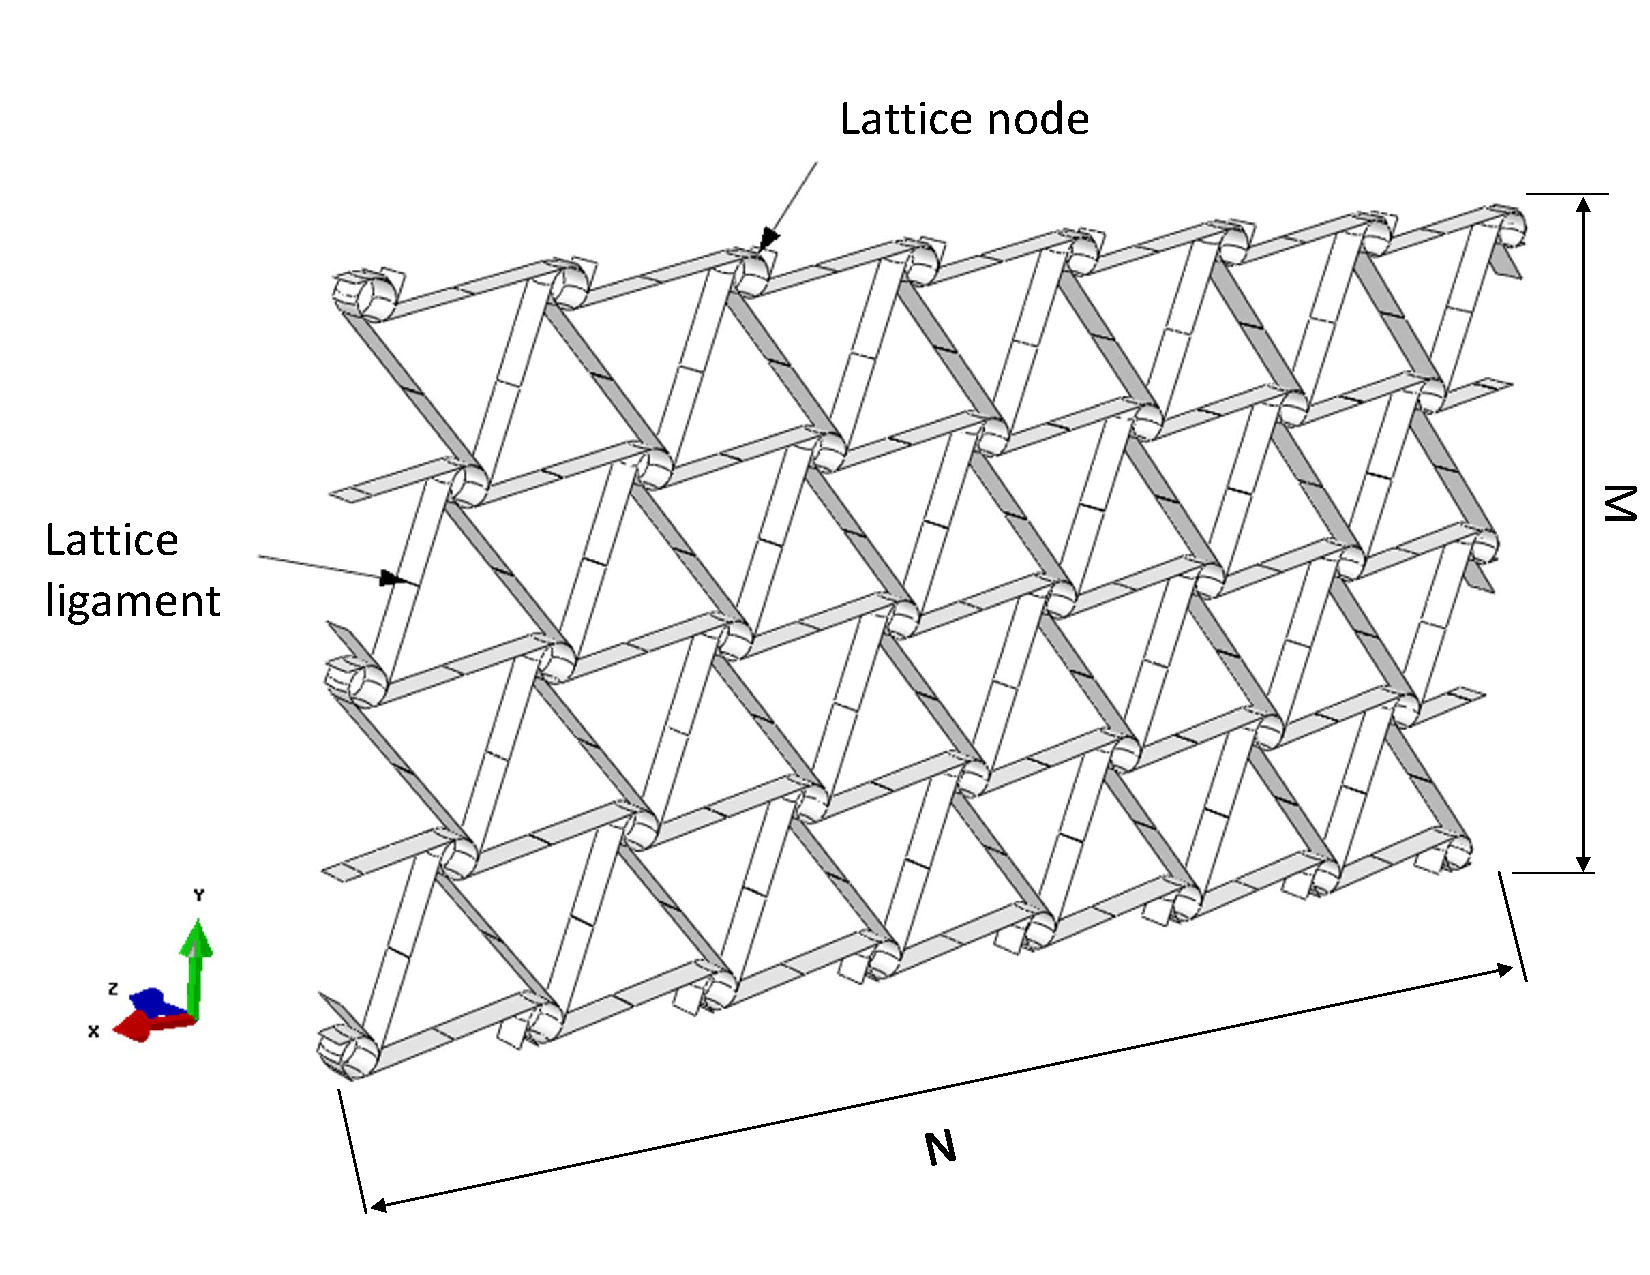
\includegraphics[width=0.8 \textwidth]{model/lattice}
  \caption[Overview of the chiral lattice part]{Overview of the chiral lattice part. The parameters $M$ and $N$ represent the number of unit cells }\label{fig:lattice}
\end{figure}

\begin{figure}[!htpb]
  \centering
  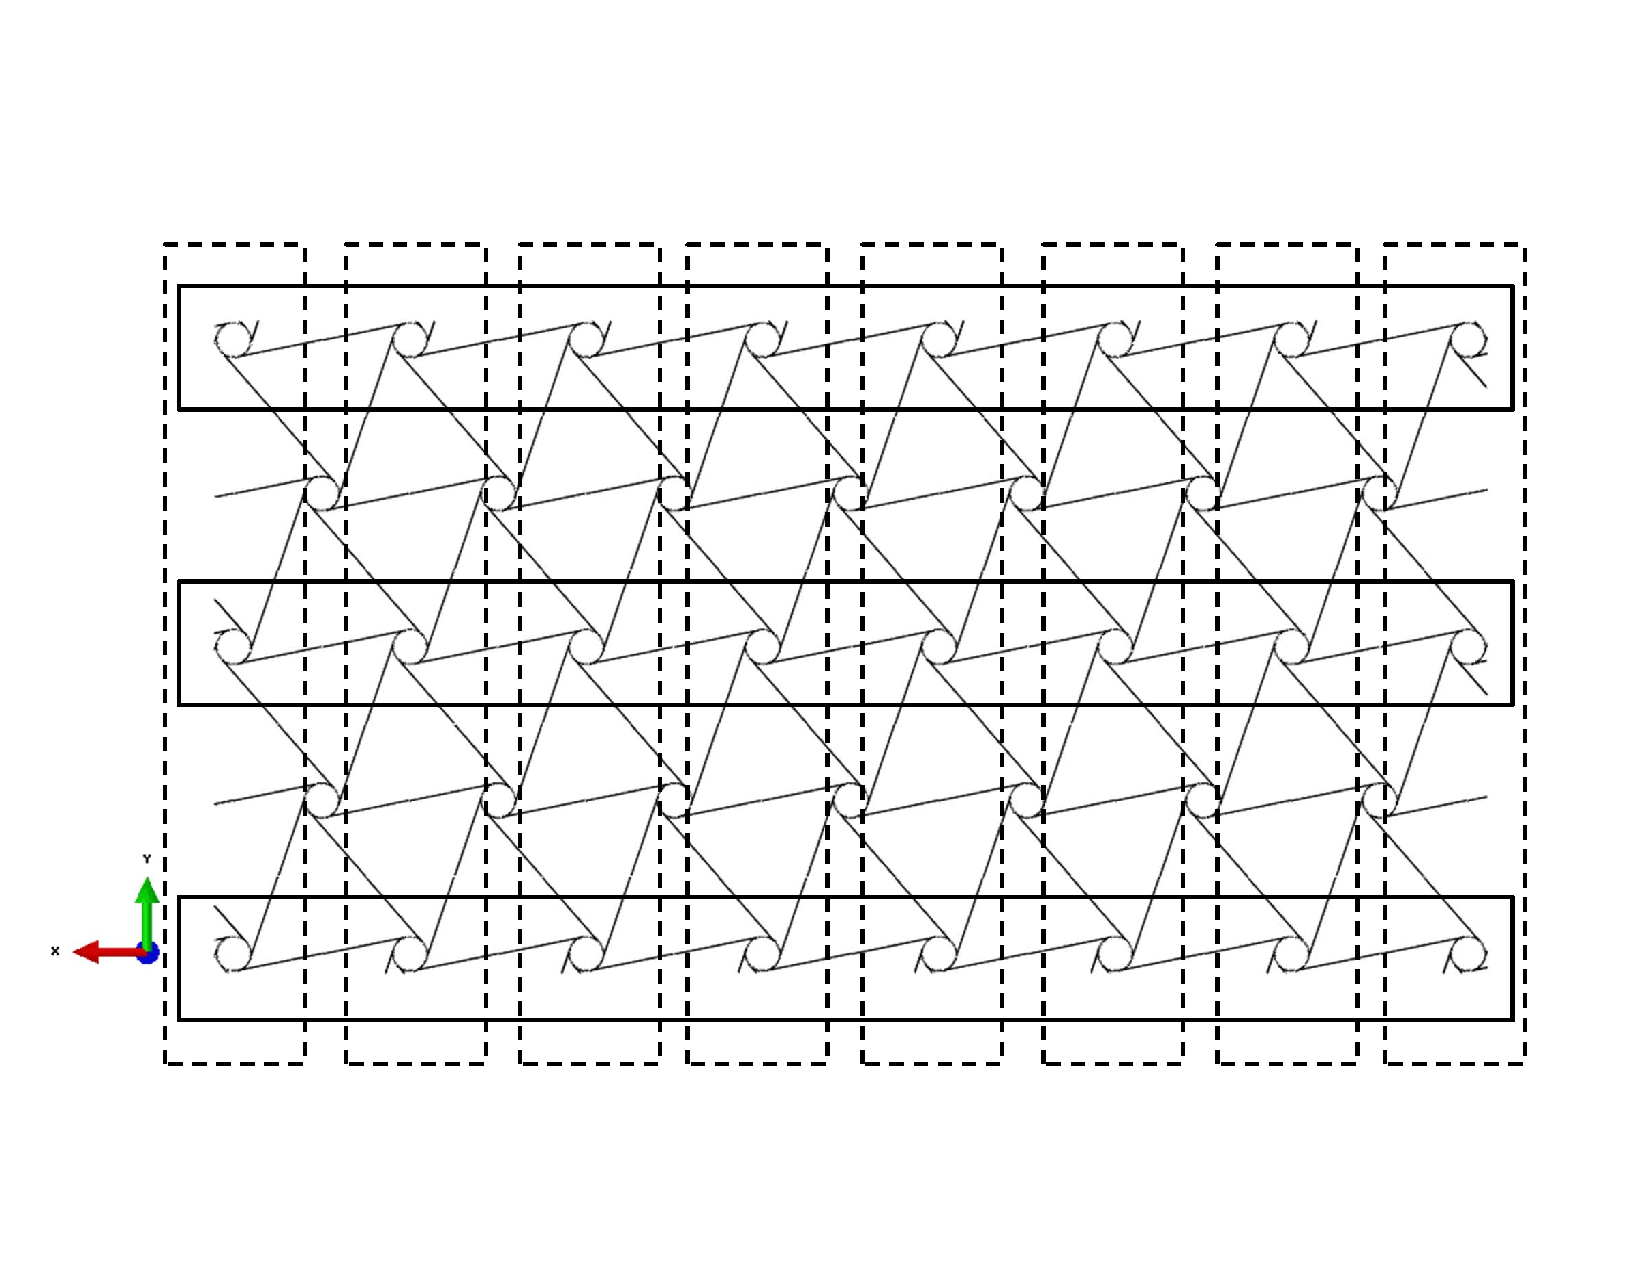
\includegraphics[width=0.8 \textwidth]{model/lattice-NandM}
  \caption[]{}\label{fig:lattice-NandM}
\end{figure}

\begin{figure}[!htpb]
  \centering
  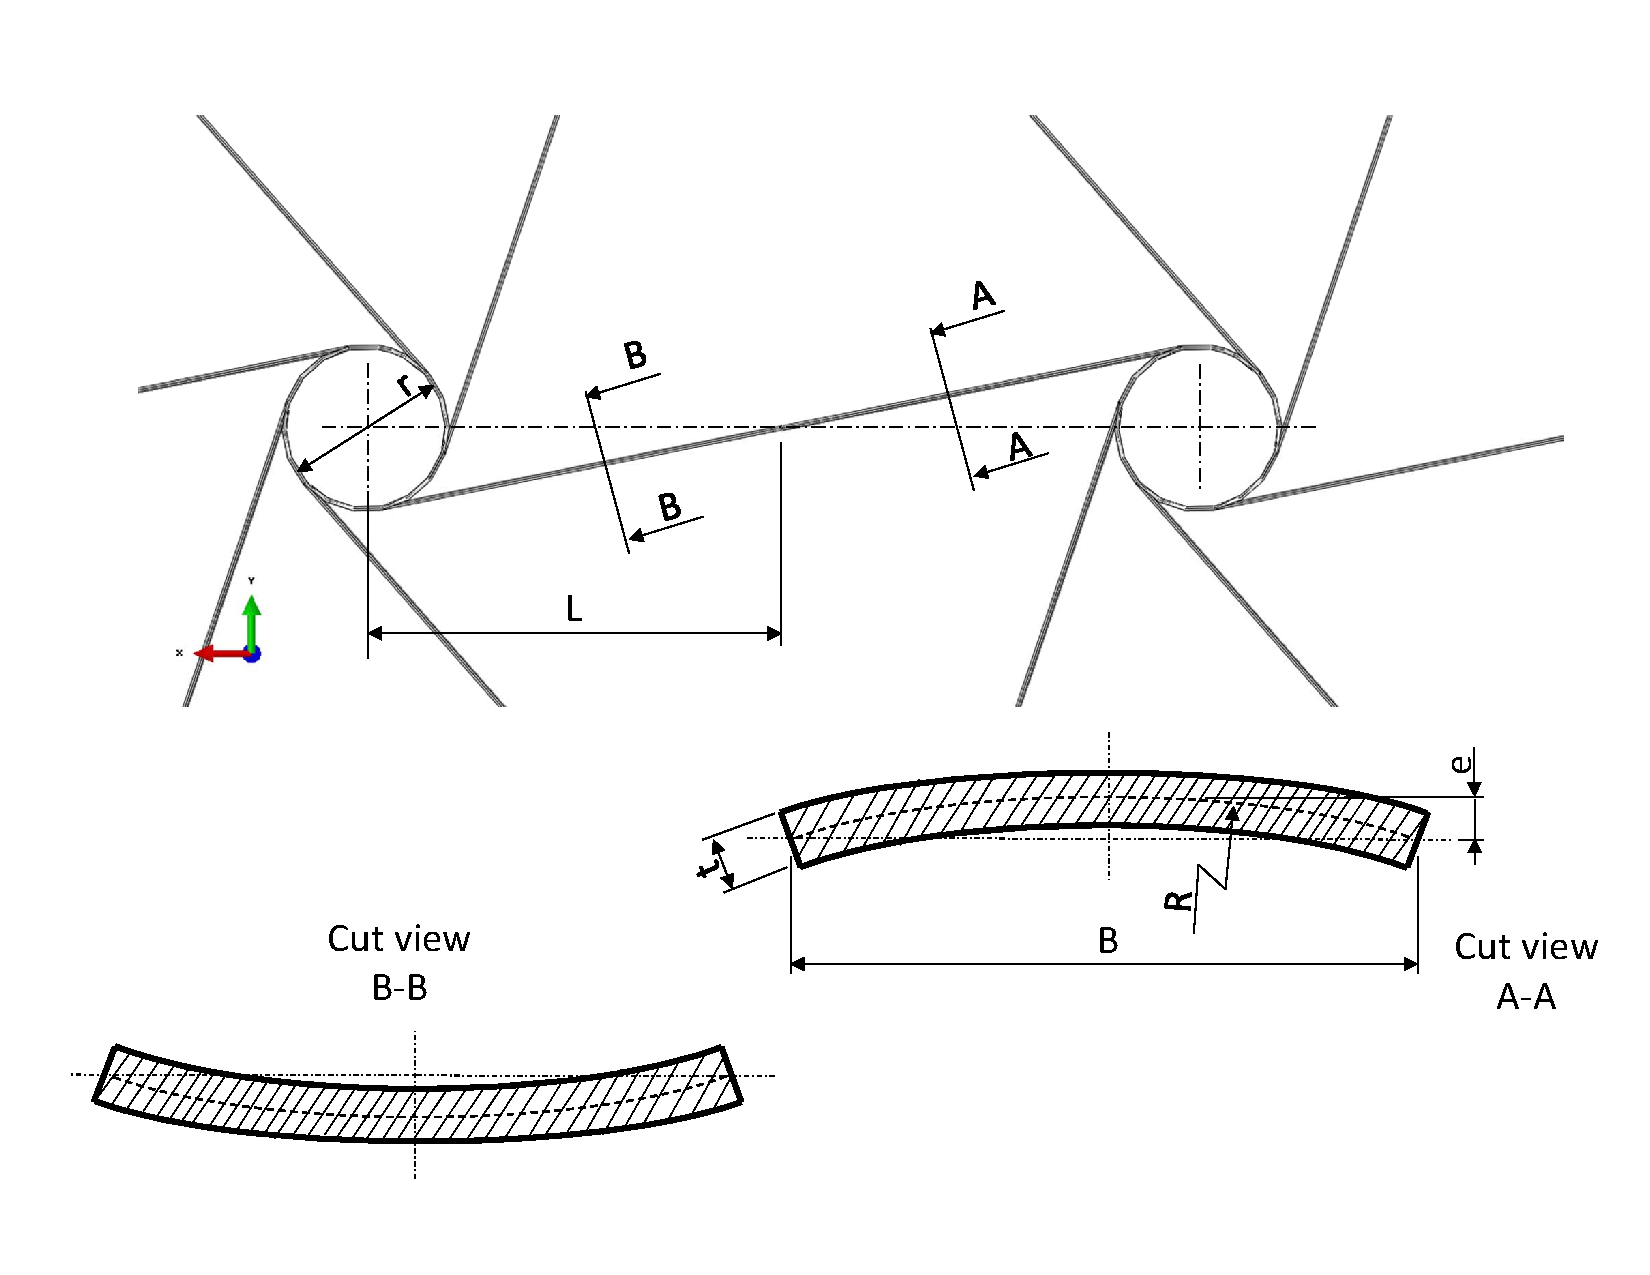
\includegraphics[width=0.8 \textwidth]{model/lattice-internalParameters}
  \caption[]{}\label{fig:lattice-internalParameters}
\end{figure}

\begin{table}[!htpb]
\centering
\begin{tabular}{|l|lll|}
\hline
\textbf{Parameter} & \multicolumn{1}{l|}{\textbf{Symbol}} & \multicolumn{1}{l|}{\textbf{Units}} & \textbf{Nominal value} \\ \hline \hline
{\textbf{Dimensions}} &  &  &  \\ \hline
Number of unit cells in spanwise direction & \multicolumn{1}{l|}{$N$} & \multicolumn{1}{l|}{} & 8 \\ \hline
Number of unit cells in transversal direction & \multicolumn{1}{l|}{$M$} & \multicolumn{1}{l|}{} & 3 \\ \hline
Dimensionless eccentricity (e/B) & \multicolumn{1}{l|}{$e_{\mathrm{chiral}}$} & \multicolumn{1}{l|}{} & 0.01 \\ \hline
Node radius & \multicolumn{1}{l|}{$r_{\mathrm{chiral}}$} & \multicolumn{1}{l|}{mm} & 10 \\ \hline
Node depth & \multicolumn{1}{l|}{$B_{\mathrm{chiral}}$} & \multicolumn{1}{l|}{mm} & 20 \\ \hline
Ligament half length & \multicolumn{1}{l|}{$L_{\mathrm{chiral}}$} & \multicolumn{1}{l|}{mm} & 50 \\ \hline \hline
{\textbf{Material (ABS)}} &  &  &  \\ \hline
Young's modulus & \multicolumn{1}{l|}{$E_{\mathrm{chiral}}$} & \multicolumn{1}{l|}{N/mm$^2$} & 31000 \\ \hline
Poisson's ratio & \multicolumn{1}{l|}{$\nu_{\mathrm{chiral}}$} & \multicolumn{1}{l|}{} & 0.3 \\ \hline
\end{tabular}
\caption[Parameters used for the lattice model]{Parameters used for the lattice model. The mechanical properties of the material used correspond to ABS, which is a common thermoplastic polymer.}
\label{tab:parameters_lattice}
\end{table}

\begin{figure}[!htpb]
  \centering
  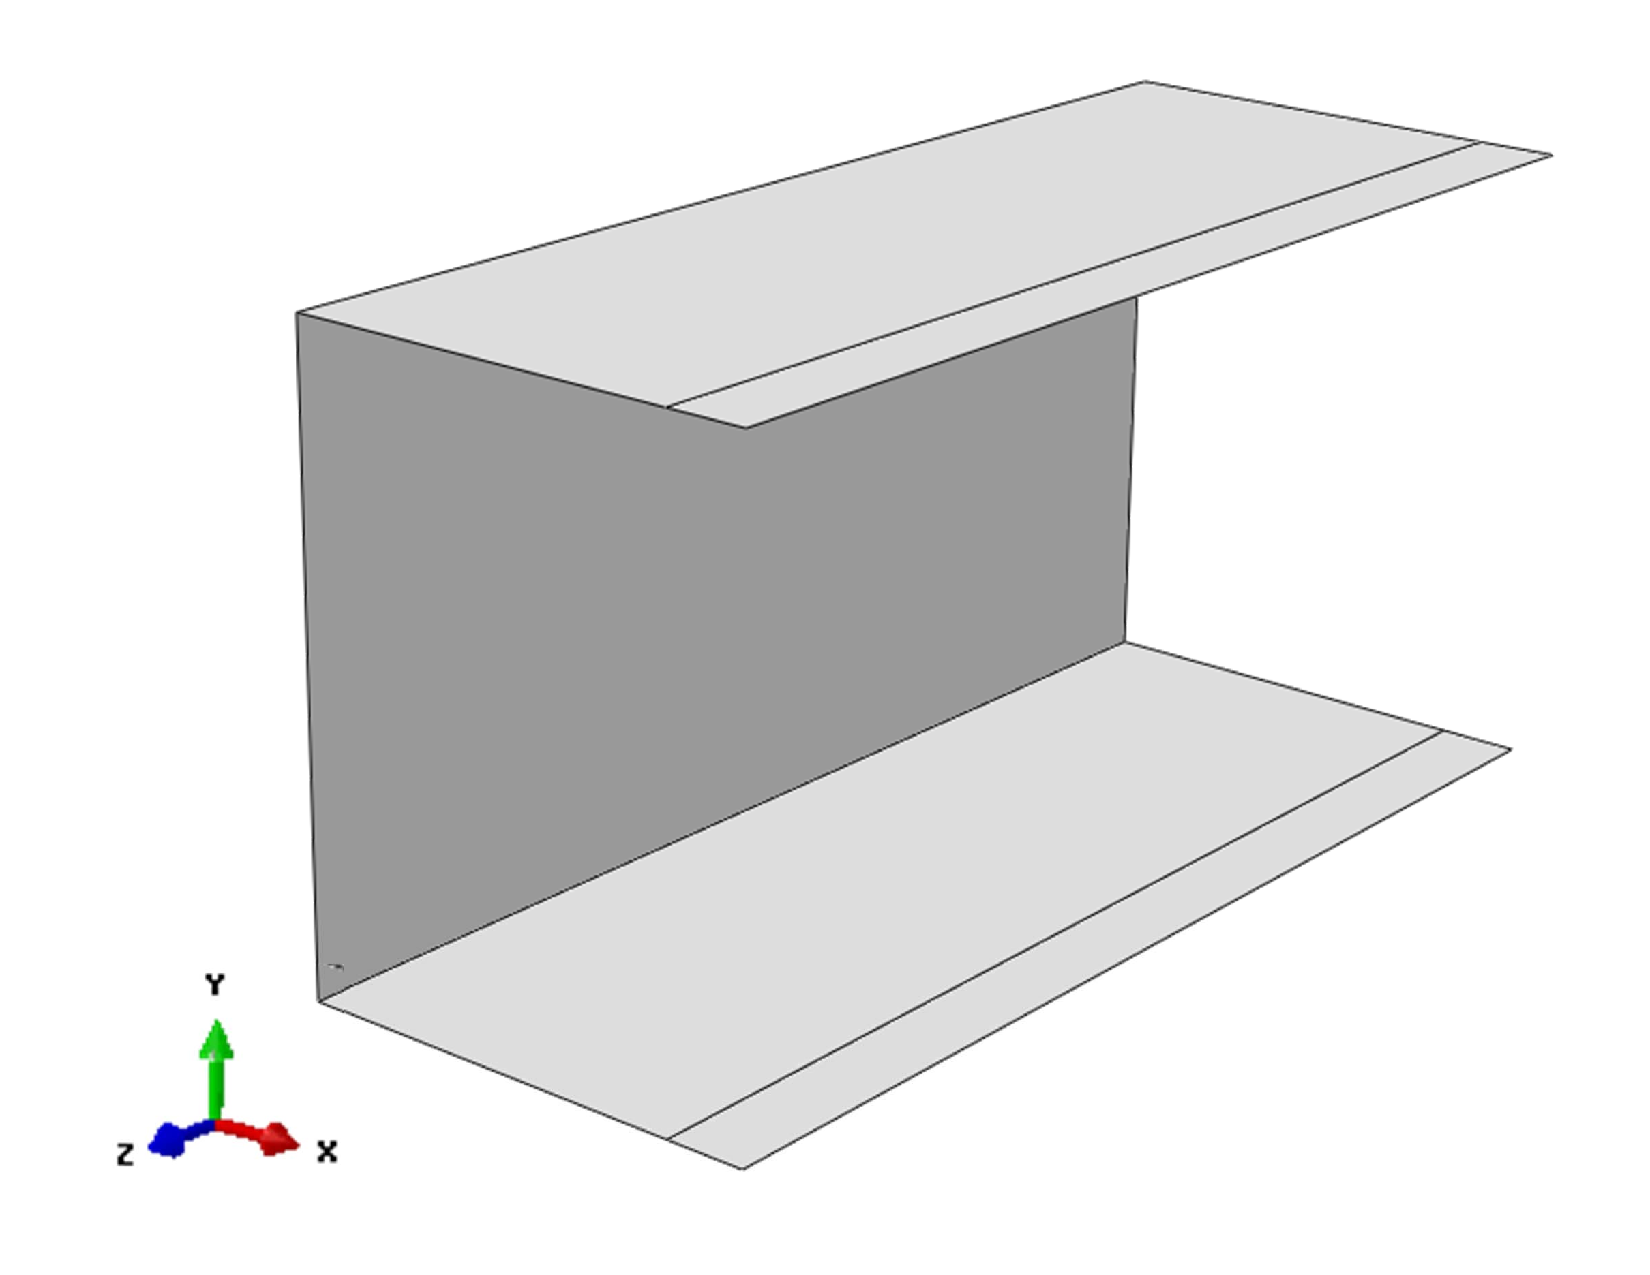
\includegraphics[width=0.8 \textwidth]{model/wing-box}
  \caption[Overview of the wing-box in C-profile part]{Overview of the wing-box in C-profile part}\label{fig:wing-box}
\end{figure}

\subsection{Attachment points modeling} \label{subsec:connections_computationalModel}

%General thoughts:
% - Necessity of applying condition node to node
%
%Equation contrainsts issues:
% - Slow down simulations
%
%Coupling constrainsts:
% 
%
In the present subsection, the FEM modeling of the connection between the lattice nodes and the wing box is presented. The connection that will be modeled is the one that can be seen in Figure XX.

%Figure provided by Rafael Vincenz

Two different connections will be modeled. Firstly, all the degrees of freedom of the lattice will be restricted except from the rotation around its own axis. An sketch showing this connection can be viewed in Figure \ref{fig:connectionModeling1}. This was the design chosen for the manufactured demonstrator shown in Figure XX.

Another option for the modeling was to leave the lattice node displacement parallel to the skin unconstrained. This allows another degree of freedom for this element and therefore the connection between the node lattice and the skin is schematically like the one shown in Figure \ref{fig:connectionModeling2}.

\begin{figure}[!htpb]
  \centering
  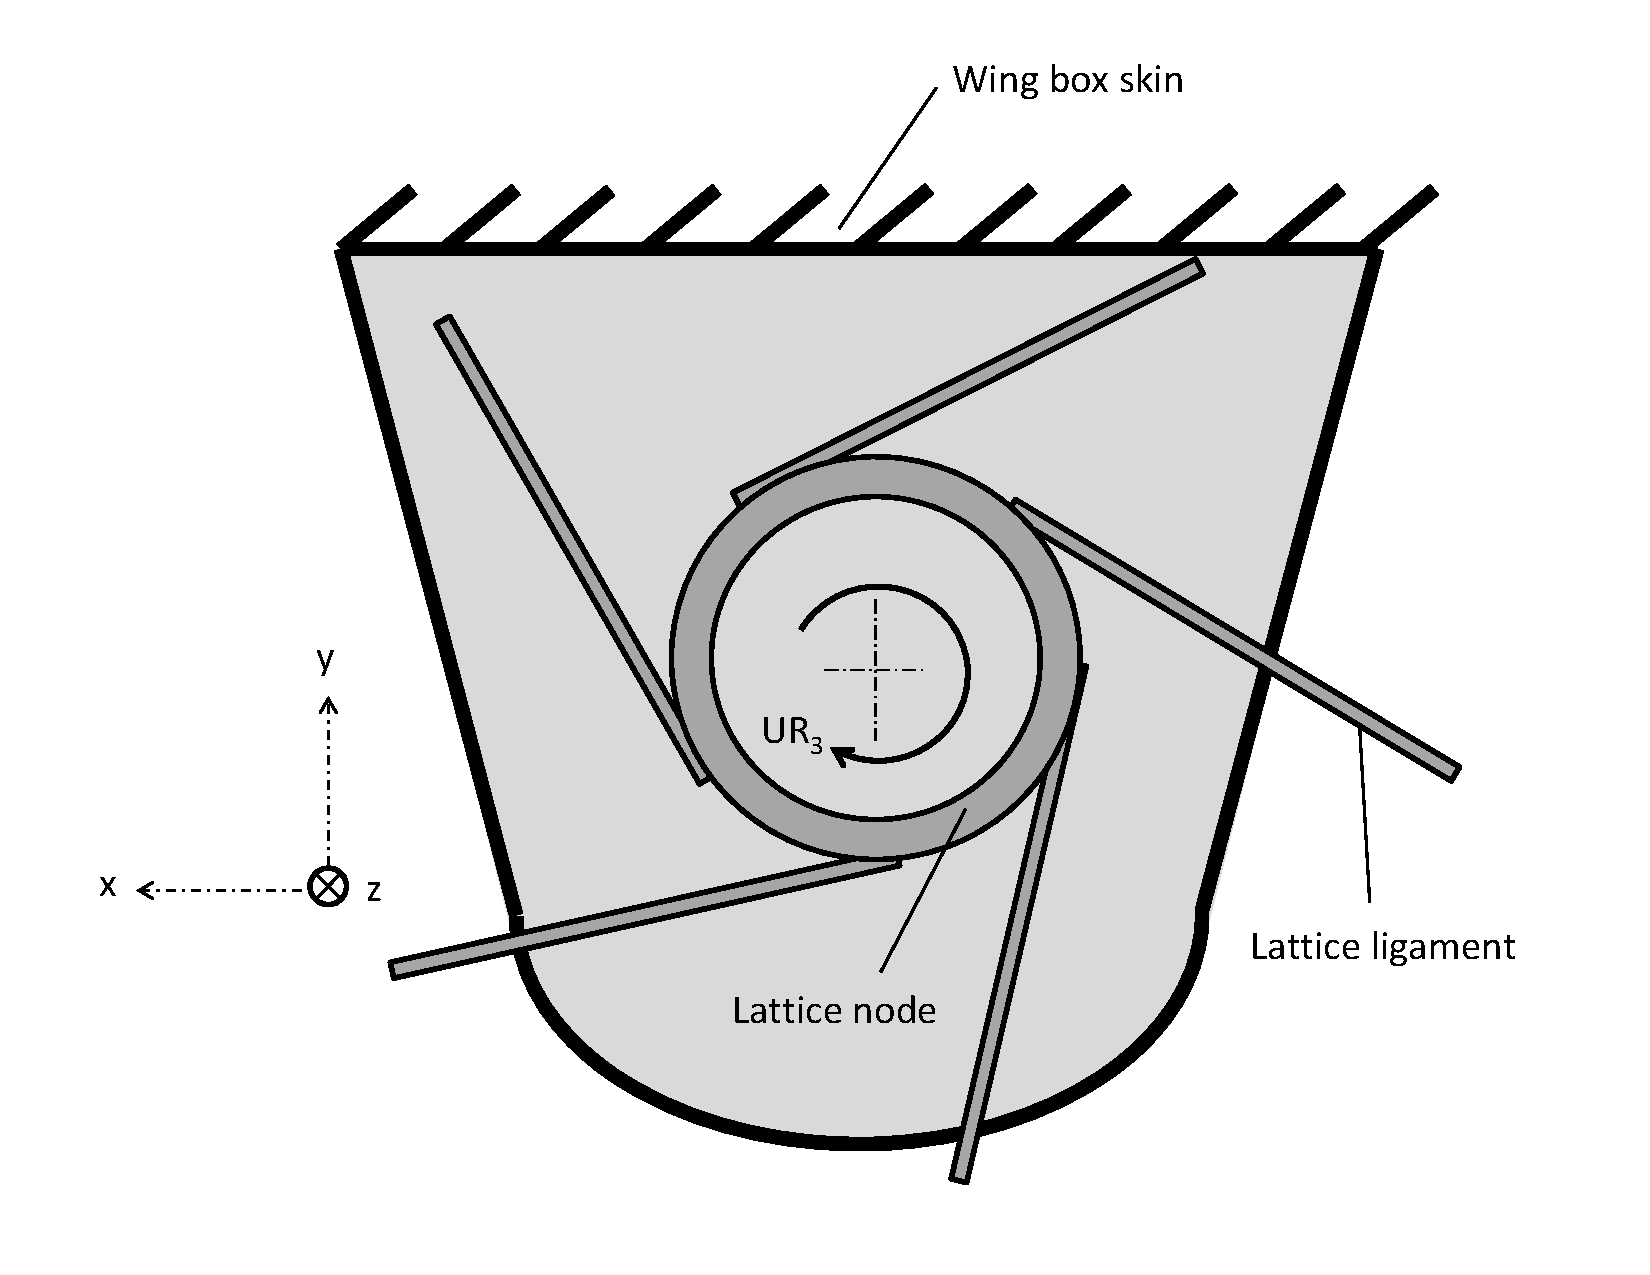
\includegraphics[width=0.8 \textwidth]{model/connectionModeling1}
  \caption[First type of connection lattice-skin considered]{First type of connection lattice-skin considered. }\label{fig:connectionModeling1}
\end{figure}

\begin{figure}[!htpb]
  \centering
  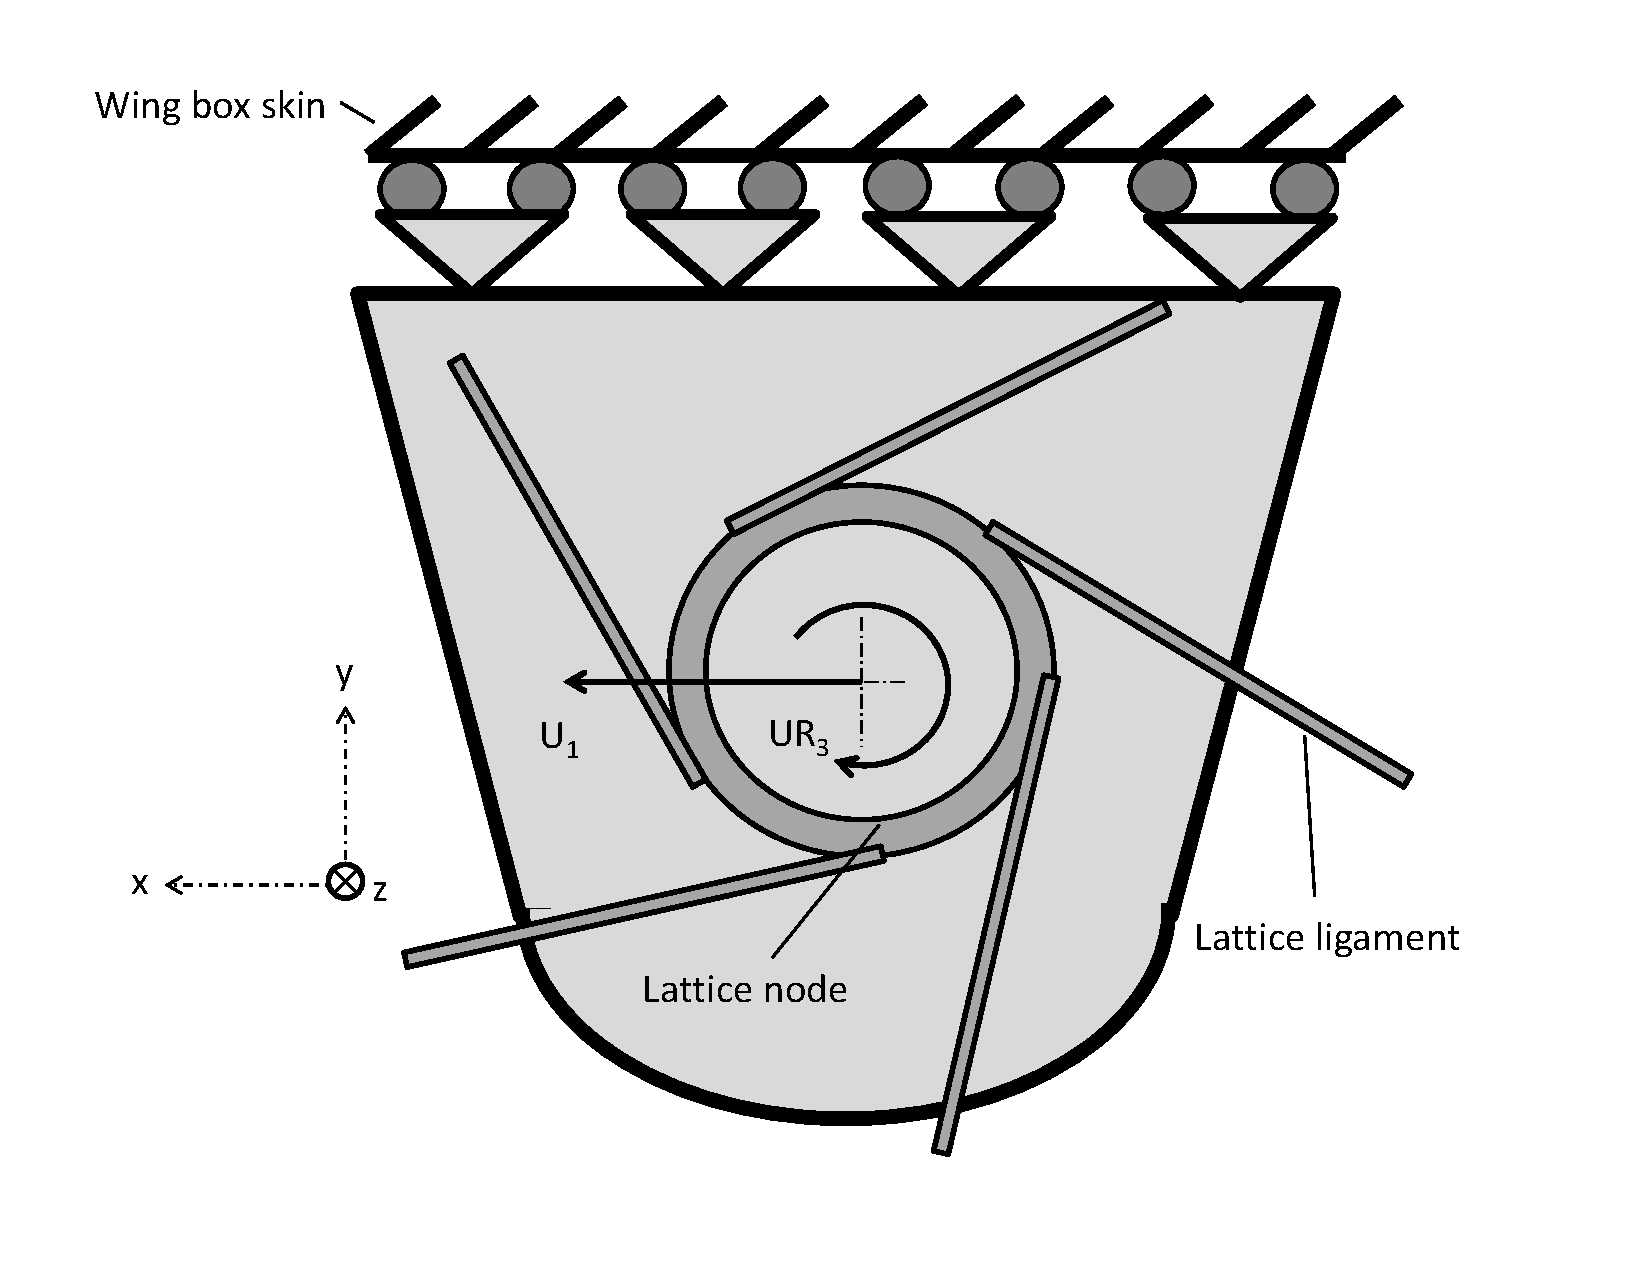
\includegraphics[width=0.8 \textwidth]{model/connectionModeling2}
  \caption[Second type of connection lattice-skin considered]{Second type of connection lattice-skin considered. }\label{fig:connectionModeling2}
\end{figure}

In order to model the connections shown in Figures \ref{fig:connectionModeling1} and \ref{fig:connectionModeling2}, different different approaches were explored. 

\subsubsection{}